\chapter{Mise en œuvre des modèles}

\section{Arbre de décision}

Nous n'avons malheureusement pas eu le temps d'effectuer cette partie.

\section{Réseaux de neurones artificiels}

Concernant cette partie, notre réseaux de neurones fonctionne, il nous manque uniquement l'implémentation de l'early-stopping. Cependant, nous allons tout de même procéder à une analyse détaillée de notre implémentation et la comparer aux résultats qui accompagnent le sujet afin de vérifier son bon fonctionnement.

Nous avons décidé d'aller plus loin en implémentant des fonctions d'initialisation de poids différentes (\texttt{xavier} et \texttt{he-et-al}). Afin de voir si l'une ou l'autre est plus intéressante à utiliser, nous avons entrainé chaque modèle une fois avec \texttt{xavier} et une autre avec \texttt{he-et-al}. Pour chaque entrainement nous avons généré les schémas de la matrice de confusion et des taux d'erreur.

Ne voulant pas surcharger, les données que nous analyserons ici ne seront pas intégrées dans ce rapport. En revanche, elles sont accessibles depuis l'archive dans \texttt{report/our-analysis}.

Pour les modèles \texttt{6-4}, on remarque que les résultats sont sensiblement similaires.
A partir des modèles \texttt{10-8-4}, on remarque que \texttt{xavier} a tendance à obtenir un nombre d'erreurs tout de même supérieur à son homologue \texttt{he-et-al}. En revanche, pour les modèles \texttt{10-8-6}, on remarque que \texttt{Relu he-et-al} performe moins bien, mais les résultats demeurent corrects.

La partie suivante est effectuée après les analyses de fin de rapport, ne voulant pas tout mélanger, nous en parlons donc ici.

De manière générale, on remarque que nos modèles \texttt{Relu} possèdent tout de même un nombre d'erreurs plus elevé que les résultats qui accompagnent le sujet. Cependant, l'inverse est facilement observable pour les modèles \texttt{Tanh}, excepté \texttt{10-8-6}. Cela ce remarque notamment grâce aux matrices de confusion.

Finalement, on remarque encore une fois que c'est le modèle \texttt{Tanh 10-8-6}, en particulier sa version \texttt{he-et-al}, qui obtient les meilleurs résultats, ce qui nous conforte dans notre analyse.

A titre d'information, voici la courbe des erreurs de ce modèle.

\begin{table}[H]
    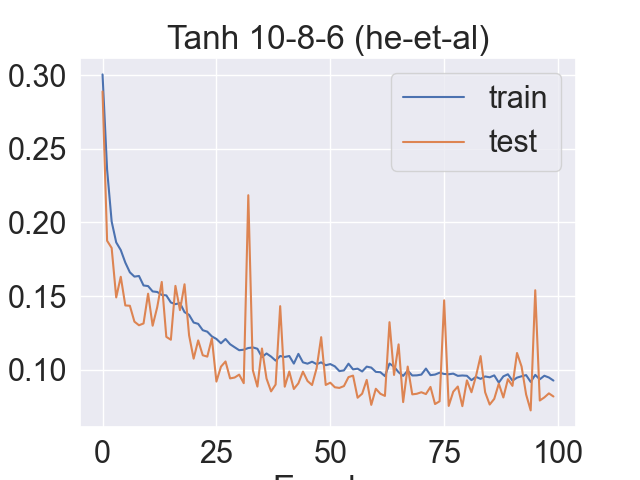
\includegraphics[scale=0.6]{images/tanh-10-8-6-errors.png}
    \caption{\label{HomePage} Schéma du taux d'erreurs en fonction de l'epoch (Tanh \texttt{10-8-6})}
\end{table}